\lab{Algorithms}{B\'{e}zier Curves}{B\'{e}zier Curves}

\objective{Understand the basics of B\'{e}zier Curves and De Casteljau's algorithm}

There are many different ways of approximating functions.
In computer graphics, spline curves are often used.

At times it may be helpful to find an approximating curve that does not depend on any particular coordinate system.
This means that by rotating the coordinate axes, we do not actually change the curve.
This is a problem with many curve interpolation methods.
Figure \ref{bezier:bad_interpolation} is an example of two interpolating curves through a set of points in different coordinate systems.

\begin{figure}
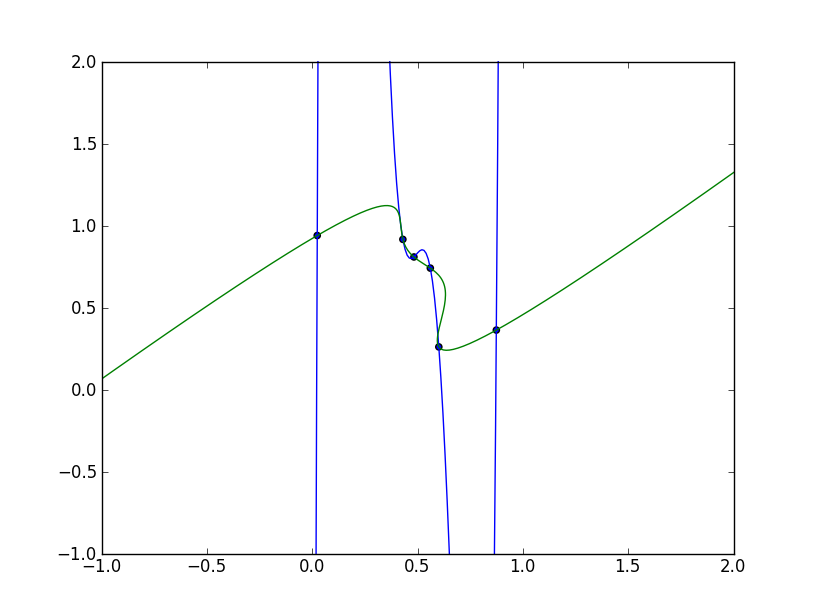
\includegraphics[width=.9\textwidth]{bad_interpolation}
\caption{Interpolation of a set of points under different coordinate systems.}
\label{bezier:bad_interpolation}
\end{figure}

Another problem with traditional interpolation is that, though the curve may pass through each point, its behavior between the points we are interpolating may be unpredictable, as in the following example.
This is called Runge's Phenomenon.
Figure \ref{bezier:bad_interpolation2} shows how Runge's phenomenon can apply to polynomial interpolation.
When approximating a function, this effect can be avoided by using carefully chosen interpolation points; however, when we are trying to approximate a given set of points, we will may not always be able to choose which points are given.
Carefully choosing interpolation points still leaves us with the rotation problem illustrated above.

\begin{figure}
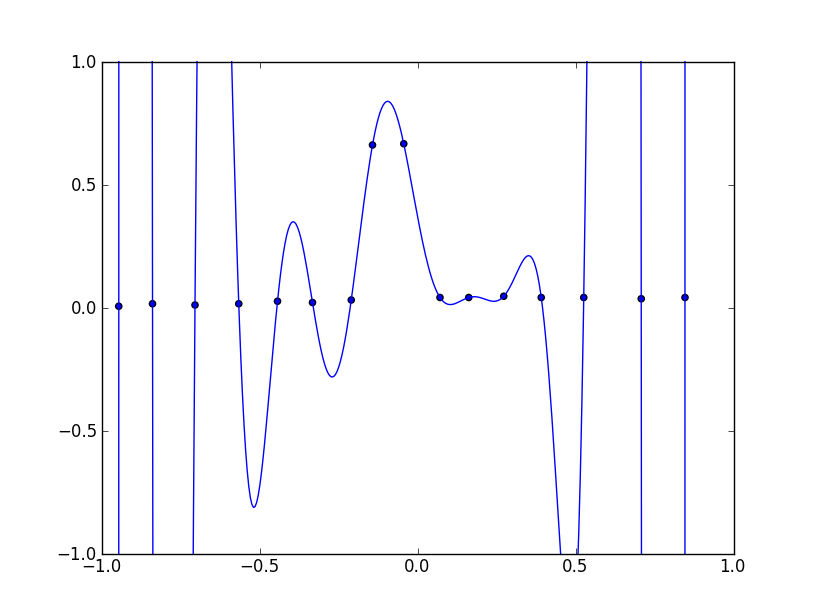
\includegraphics[width=.9\textwidth]{bad_interpolation2}
\caption{A simple example of Runge's phenomenon in polynomial interpolation.}
\label{bezier:bad_interpolation2}
\end{figure}

Ideally, we should be able to find a more stable curve that can be easily manipulated to fit the shape we want.
This is why B\'{e}zier curves were invented.
The following is a geometric way of tracing out a B\'{e}zier curve for an ordered set of $n$ points.
These are called control points.
We would like to define a smooth curve from the first point to the last point which can be manipulated according to the position of the other points.
We will parameterize this curve between the first and last point with respect to $t$, letting $t$ go from $0$ to $1$.
To evaluate the curve at a given time $T_0$ do the following:
\begin{itemize}

\item

Parameterize the lines between each of the points letting $t$ go from $0$ to $1$.
For the points $P_{n}$ and $P_{n+1}$ this parameterization is $P_{n} (1-t) + P_{n+1} t$.

\item

Evaluate each of these parameterizations at $T_0$.
Note that this gives $n-1$ new points.

\item

Repeat this process on the list of points until only one point is left.
This is the value of the B\'{e}zier curve for these control points at the parameter $T_0$.

\end{itemize}

This is what is known as De Casteljau's Algorithm. 
It can be illustrated as follows:

Figures \ref{bezier:decasteljau_1} through \ref{bezier:decasteljau_5} are illustrations of De Casteljau's Algorithm for $4$ points at $t= 0$, $.25$, $.5$, $.75$, and $1$ respectively.

\begin{figure}
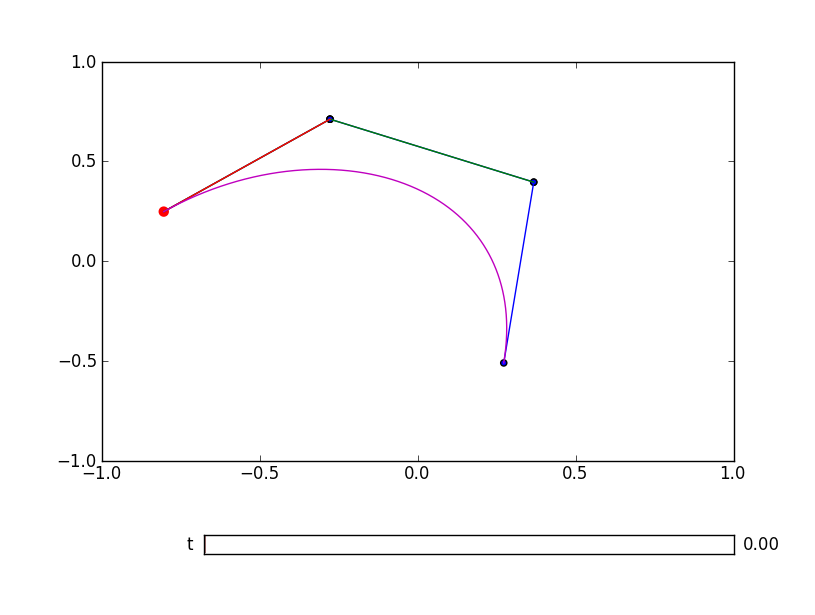
\includegraphics[width=\textwidth]{decasteljau_1}
\caption{An illustration of the Decasteljau Algorithm at $t=0$.}
\label{bezier:decasteljau_1}
\end{figure}

\begin{figure}
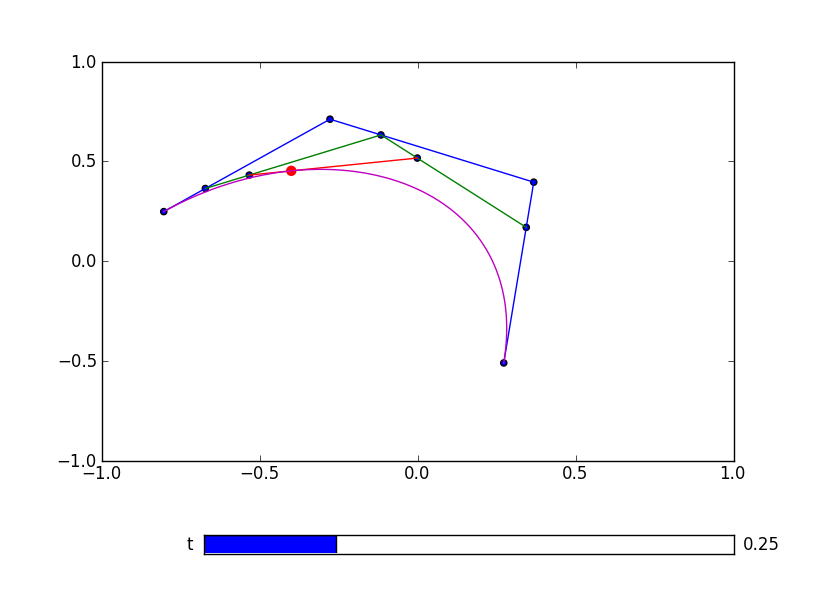
\includegraphics[width=\textwidth]{decasteljau_2}
\caption{$t=.25$}
\label{bezier:decasteljau_2}
\end{figure}

\begin{figure}
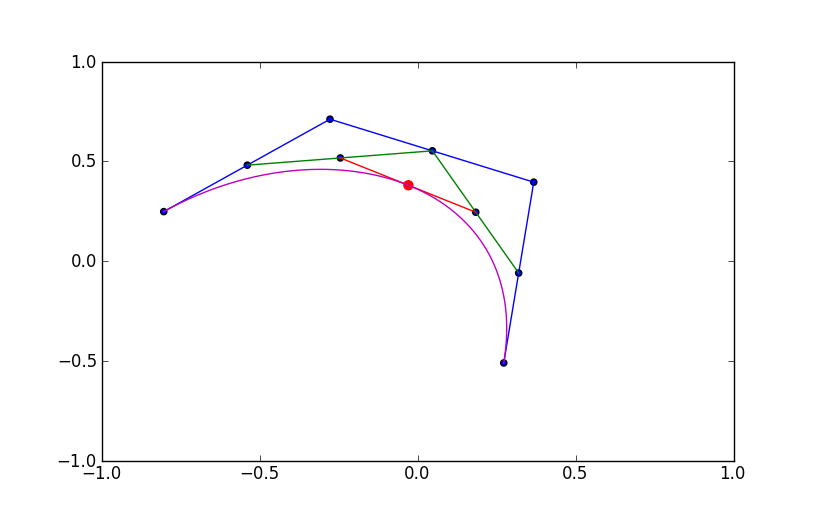
\includegraphics[width=\textwidth]{decasteljau_3}
\caption{$t=.5$}
\label{bezier:decasteljau_3}
\end{figure}

\begin{figure}
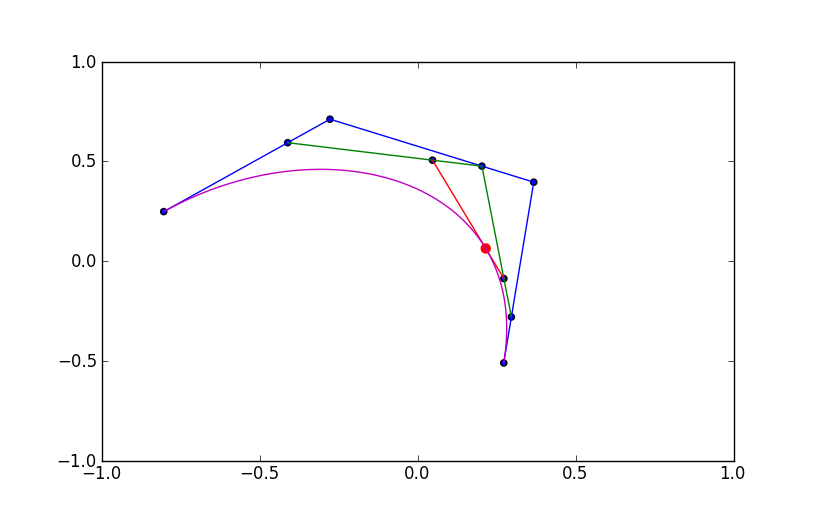
\includegraphics[width=\textwidth]{decasteljau_4}
\caption{$t=.75$}
\label{bezier:decasteljau_4}
\end{figure}

\begin{figure}
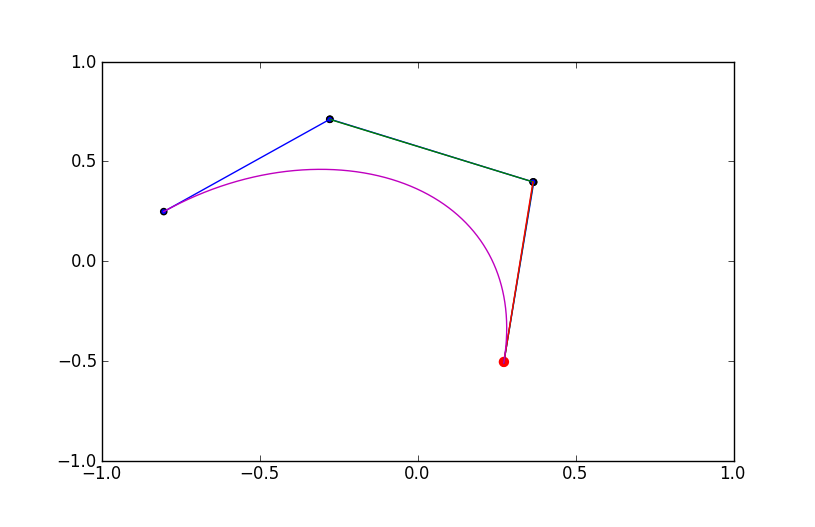
\includegraphics[width=\textwidth]{decasteljau_5} 
\caption{$t=1$.}
\label{bezier:decasteljau_5}
\end{figure}

This algorithm works for large numbers of points, though evaluation time increases rapidly.
Figure \ref{fig:bezier:decasteljau_many_points}

\begin{figure}
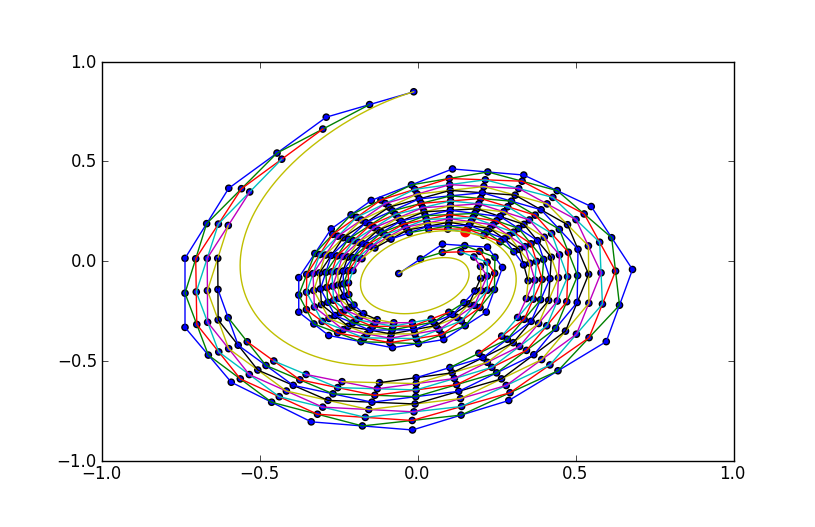
\includegraphics[width=\textwidth]{decasteljau_6}
\caption{An illustration of the Decasteljau Algorithm for a higher number of points.}
\label{fig:bezier:decasteljau_many_points}
\end{figure}

\begin{problem}
Implement De Casteljau's algorithm.
Have your function accept a $m \times n$ array representing $m$ control points.
Also have it accept a time $t$ at which to evaluate the curve.
\end{problem}

\begin{comment}
% this is cool, but it isn't core to the algorithm.
\begin{problem}
Use a slider bar to interactively show how the algorithm works.
Use Matplotlib's \li{ginput} function to get the control points for the graph.
\end{problem}
\end{comment}

Notice that these curves depend on the points themselves and not on the coordinate system with which we are viewing them.
Since a B\'{e}zier curve is defined entirely by convex combinations of its control points, we can rotate the coordinate system without changing the shape of the curve.

\begin{figure}
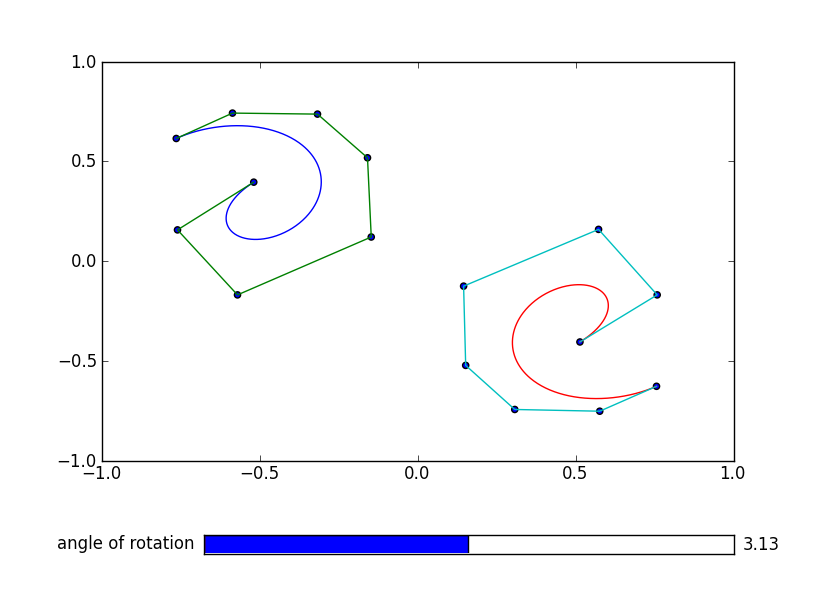
\includegraphics[width=\textwidth]{bezier_rotation}
\caption{B\'{e}zier curves do not change under rotation.
These two different curves (and their corresponding control points) are exact rotations of one another.}
\end{figure}

There is a way of generating these functions explicitly.
Each of the coordinate functions of a curve can be written as sums of Bernstein polynomials in $t$.
The $k$'th Bernstein polynomial of order $n$ is written as

$$\theta_{i,n}=\left( \begin{smallmatrix} n\\ i \end{smallmatrix} \right) (1-t)^{n-i} t^i$$

where $\left( \begin{smallmatrix} n\\ i \end{smallmatrix} \right) = \frac{n!}{i!(n-i)!}$, i.e. the binomial coefficients.

\begin{info}
You don't need to compute the binomial coefficients directly.
Scipy includes the function \li{scipy.misc.comb} to compute the binomial coefficients.
\end{info}

The B\'{e}zier curve for a given set of control points (also called the control polygon) is given by the formula:

$$\gamma (t) = \sum_{i=0}^n P_i \theta_{i,n} (t)$$

where $P_i$ is the i'th point of the control polygon.

These functions are convenient for quick evaluation of low order B\'{e}zier curves, but they are not stable for high numbers of points.
This is because the coefficients $\left( \begin{smallmatrix} n\\ i \end{smallmatrix} \right)$ for some of the terms of each polynomial grow very rapidly for large $n$.
For example, $\left( \begin{smallmatrix} 40\\ 20 \end{smallmatrix} \right)=137846528820$.
The errors that can come from having these large coefficents used in each of these polynomials do not cause any trouble for low degree polynomials, but they quickly become a concern for polynomials with higher degrees.

\begin{problem}
Write a function that, given the numbers $i$ and $n$, returns the $i$'th Bernstein polynomial of degree $n$.
Use a NumPy \li{poly1d} object to return the result.
\end{problem}

\begin{problem}
Write a python function which, given a control polygon in $2$ dimensions, returns functions for the parameterizations of $x$ and $y$.
Make each coordinate function a \li{poly1d} object.
\end{problem}

\begin{problem}
Plot a B\'{e}zier curve with 30 randomly generated control points using De Casteljau's Algorithm.
Try doing it with Bernstein polynomials.
What do you observe?
How many control points can you use before the Bernstein polynomial approach breaks down?

Compare computation time for computing different orders of B\'{e}zier curves using both methods.
For different orders of B\'{e}zier curves, try running a single point through the algorithm and running a large number of points through the algorithm.
What do you observe?
\end{problem}

\begin{comment}
\begin{problem}
Use your implementation of De Casteljau's algorithm to make a $20\times 20$ grid of B\'{e}zier curves representing the surface $sin(xy)$ on $[-\pi,\pi]\times [-pi,\pi]$.
Use the points where the gridlines intersect as the control points for each curve.
What do you observe?
\end{problem}
\end{comment}

B-splines are a generalization of B\'{e}zier curves.
They will be discussed in greater detail in Lab 
They are essentially pieciewise polynomials defined using Bernstein polynomials of lower degrees.
They allow for the easy approximation of lines with more contorol points without the extra costs that come from higher order B\'{e}zier curves.
They also make it so that a change in a single control point only chages a portion of the curve instead of forcing regeneration of the entire curve.
